\chapter{Cycle-Canceling-Algorithmus}
Für das Maximale-Fluss-Problem existiert der Ford-Fulkerson Algorithmus, welchen wir bereits kennengelernt haben. Dieser Algorithmus kann so angepasst werden, dass dieser auch für die Berechnung eines kostenminimalen Flusses benutzt werden kann. Die Anpassung sieht wie folgt aus: Anstatt mit einem $(s, t)$-Fluss zu starten, beginnt man mit einem $b$-Fluss. Nun berechnet man in jeder Iteration einen $f$-augmentierten Zykel mit negativen Kosten, wodurch man als Ergebnis einen kostenminimalen Fluss bekommt. Der Algorithmus, der genau dieses Prinzip verwendet, ist der Cycle-Canceling-Algorithmus.

\begin{table}[h!]
\setlength{\tabcolsep}{20pt}
\centering
\begin{tabular}{p{2.5cm} >{\setstretch{1.5}}p{10cm}}
\toprule
\multicolumn{2}{l}{\textbf{Cycle-Canceling-Algorithmus}} \\ \midrule
%\onehalfspacing
Input:          &Gerichteter Graph G = (V, E), obere Kapazitäten u, Kantenkosten c, Balance b.\\
 ~ & ~ \\
Output:         &Kostenminimaler Fluss f .\\
 ~ & ~ \\
Schritt 1:      &Berechnen Sie einen b-Fluss.\\
Schritt 2:      &Bestimmen Sie $G^f$ , $u^f$ und $c^f$ .\\
Schritt 3:      &Konstruieren Sie einen f -augmentierenden Zykel $Z$ in $G^f$ mit negativen Kosten. Falls keiner existiert: STOPP.\\
Schritt 4:      &Verändern Sie den b-Fluss $f$ entlang des Zykels $Z$ um $\gamma := min_{e \epsilon Z} u^f (e)$.\\
Schritt 5:      &Gehen Sie zu Schritt 2 \\
                &              \\ \bottomrule  
\end{tabular}
\label{tab: cycle_canceling_algorithmus}
\caption{Cycle-Canceling-Algorithmus}
\end{table}

\section{Berechnung eines Beispielgraphen mit dem Cycle-Canceling-Algorithmus}

Im Folgenden wird die Berechnung eines kostenminimalen Flusses $f$ anhand des Beispielgraphen in Abbildung \ref{fig:cc_step1} beschrieben.
\begin{figure}[htb]
\centering
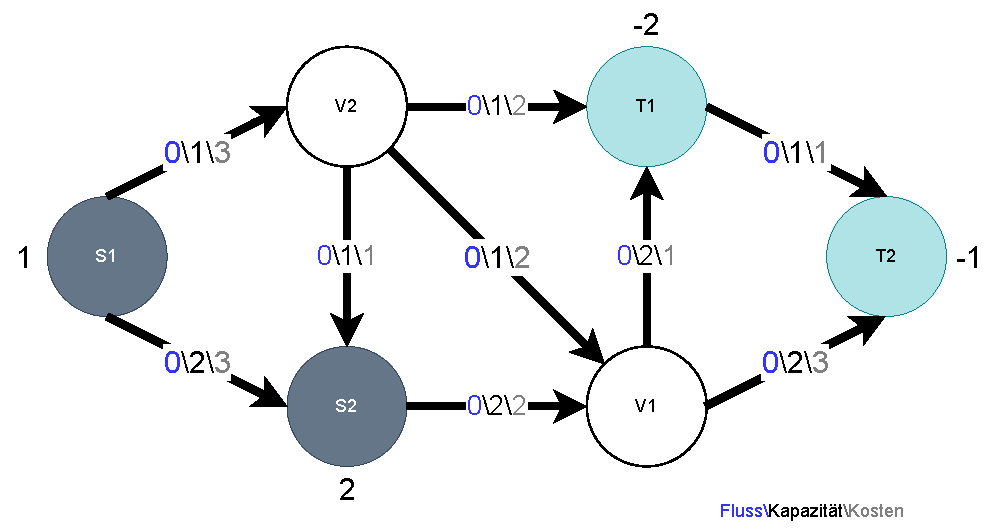
\includegraphics[width=0.7\textwidth]{img/leo/graph1-Page-1.drawio.pdf}
\caption{Cycle-Canceling-Algorithmus Schritt 1}
\label{fig:cc_step1}
\end{figure}

Im ersten Schritt des Cycle-Canceling-Algorithmuses wird ein gültiger $b$-Fluss berechnet (vgl. Abbildung \ref{fig:cc_step2}).
\begin{figure}[htb]
\centering
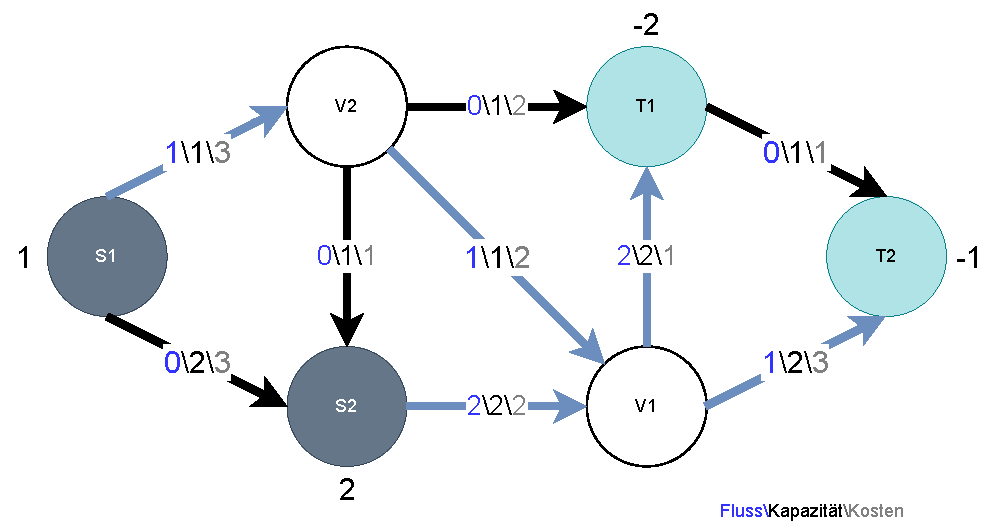
\includegraphics[width=0.7\textwidth]{img/leo/graph1-Page-2.drawio.pdf}
\caption{Cycle-Canceling-Algorithmus Schritt 2}
\label{fig:cc_step2}
\end{figure}

Im nächsten Schritt erzeugen wir zu dem in Schritt 1. bestimmten Graphen den Residualgraph mit $u^f$ und $c^f$ (vgl. Abbildung \ref{fig:cc_step3}).
\begin{figure}[htb]
\centering
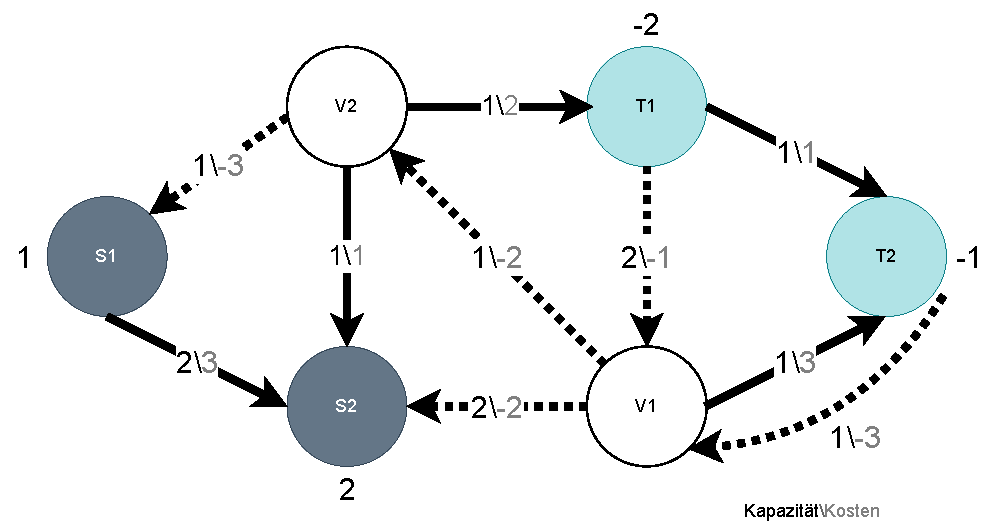
\includegraphics[width=0.7\textwidth]{img/leo/graph1-Page-3.drawio.pdf}
\caption{Cycle-Canceling-Algorithmus Schritt 3}
\label{fig:cc_step3}
\end{figure}

In Schritt 3. betrachten wir den Residualgraphen mit $u^f$ und $c^f$ und suchen in diesem nach einem Zykel, der negative Kosten hat. Gibt es keinen, sind wir mit unsrem Algorithmus fertig. In unserem Beispiel wird jedoch ein negativer Zykel mit den Kosten $-1$ von den Kanten zwischen den Knoten $V1$, $V2$ und $T1$ gebildet (vgl. Abbildung \ref{fig:cc_step4}).
\begin{figure}[htb]
\centering
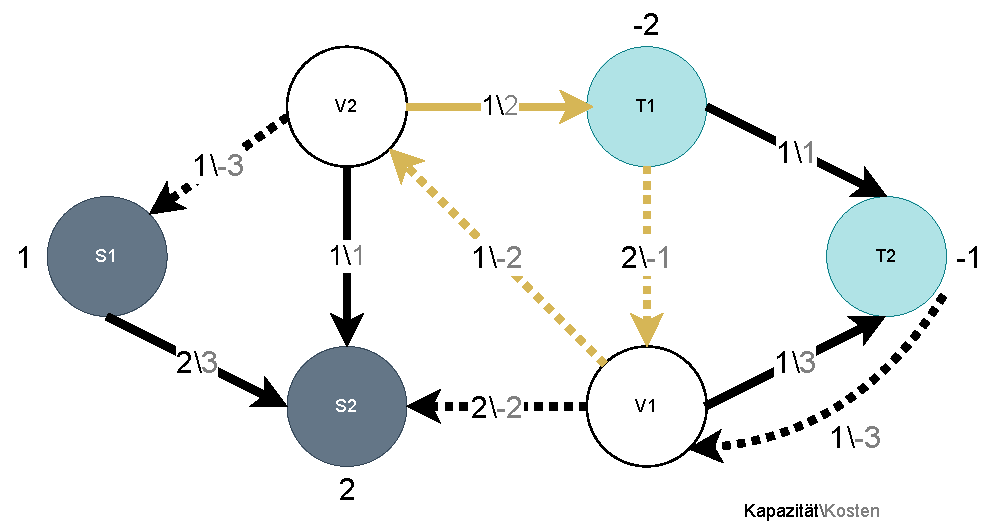
\includegraphics[width=0.7\textwidth]{img/leo/graph1-Page-4.drawio.pdf}
\caption{Cycle-Canceling-Algorithmus Schritt 4}
\label{fig:cc_step4}
\end{figure}

In Schritt 4. passen wir nun mithilfe dieses negativen Zykles unseren $b$-Fluss aus Abbildung \ref{fig:cc_step2} an. Um die Anpassung vorzunehmen, müssen wir erst die minimale Kapazität der Kanten in unserem Zykel finden. Diese minimale Kapazität ist unser $\gamma$. In unserem Fall ist $\gamma = 1$. Nun gilt haben wir im Residualgraphen eine Rückwärtskante für den Zykel benutzt, so ziehen wir unser $\gamma$ von Flusswert im ursprünglichen Graphen ab. Haben wir eine Vorwärtskante benutzt, so erhöhen wir unseren Flusswert im ursprünglichen Graphen um $\gamma$. Allgemein gilt die Definition \ref{def:augmented_cycle}. Der in unserem Beispiel entstehende Graph ist in Abbildung \ref{fig:cc_step5} zu sehen.
\begin{figure}[htb]
\centering
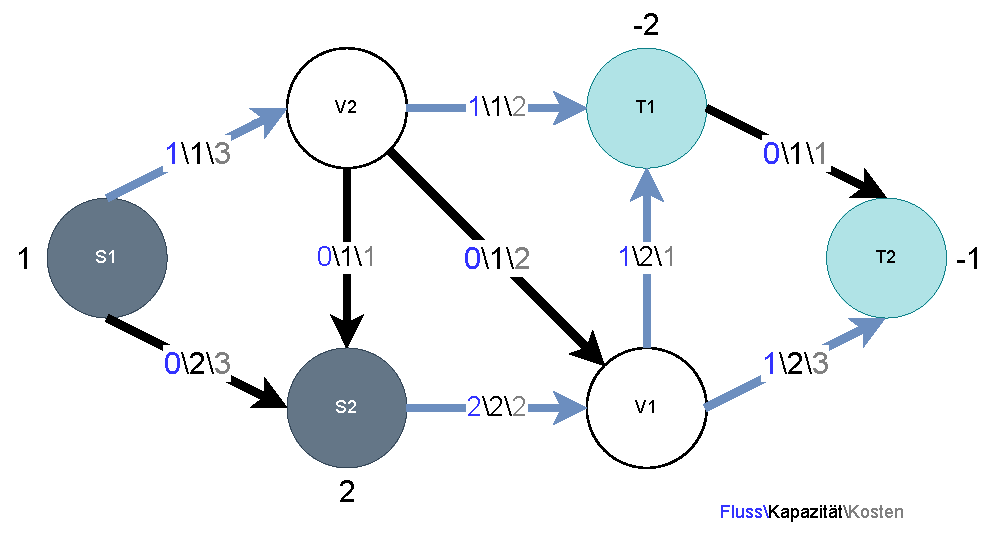
\includegraphics[width=0.7\textwidth]{img/leo/graph1-Page-5.drawio.pdf}
\caption{Cycle-Canceling-Algorithmus Schritt 5}
\label{fig:cc_step5}
\end{figure}

Zu dem neu erzeugten Graphen aus Schritt 4. wiederholen wir nun Schritt 2. Wir erzeugen erneut den Residualgraph mit $u^f$ und $c^f$ (vgl. Abbildung \ref{fig:cc_step6}).
\begin{figure}[htb]
\centering
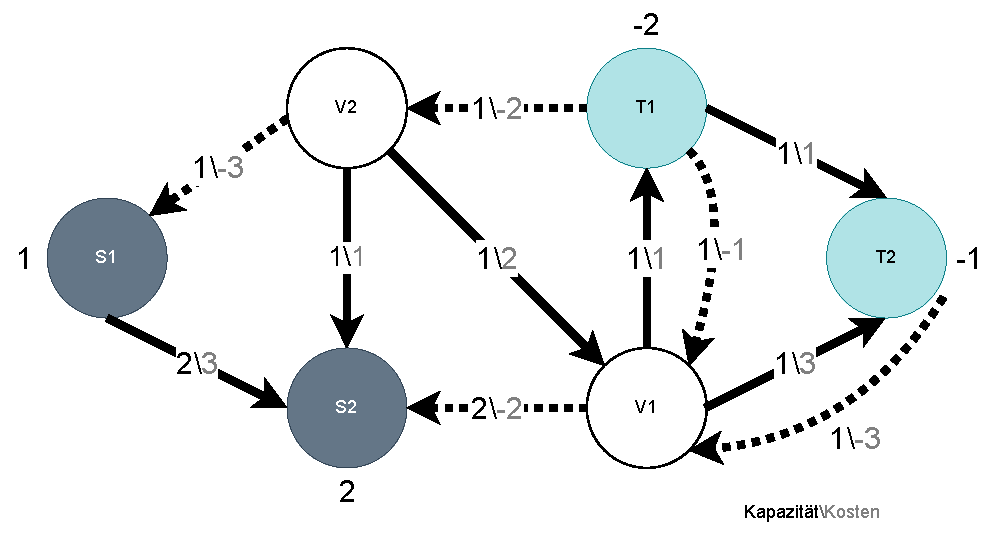
\includegraphics[width=0.7\textwidth]{img/leo/graph1-Page-6.drawio.pdf}
\caption{Cycle-Canceling-Algorithmus Schritt 6}
\label{fig:cc_step6}
\end{figure}

Nun gehen wir wieder zu Schritt 3. über und versuchen einen $f$-augmentierenden Zykel $Z$ in $G^f$ mit negativen Kosten zu konstruieren. In unserem Beispiel ist der neue Zykel nun bildbar mit den Kanten zwischen den Knoten von $T1$, $T2$ und $V1$. Der Zykel hat die Kosten $-1$ (vgl. Abbildung \ref{fig:cc_step7}).
\begin{figure}[htb]
\centering
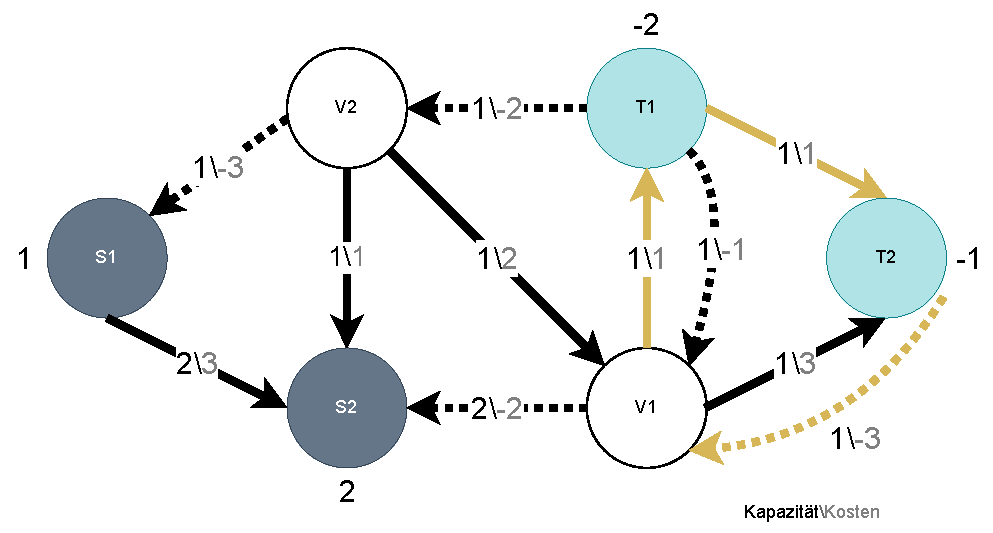
\includegraphics[width=0.7\textwidth]{img/leo/graph1-Page-7.drawio.pdf}
\caption{Cycle-Canceling-Algorithmus Schritt 7}
\label{fig:cc_step7}
\end{figure}

Im nächsten Schritt können wir nun wieder unseren ursprünglichen $b$-Fluss verändern. Dies tun wir wieder entlang des Zykels $Z$ um $\gamma := min_{e \epsilon Z} u^f (e)$. Der in unserem Beispiel neue entstehende $b$-Fluss ist in Abbildung \ref{fig:cc_step8} zu sehen.
\begin{figure}[htb]
\centering
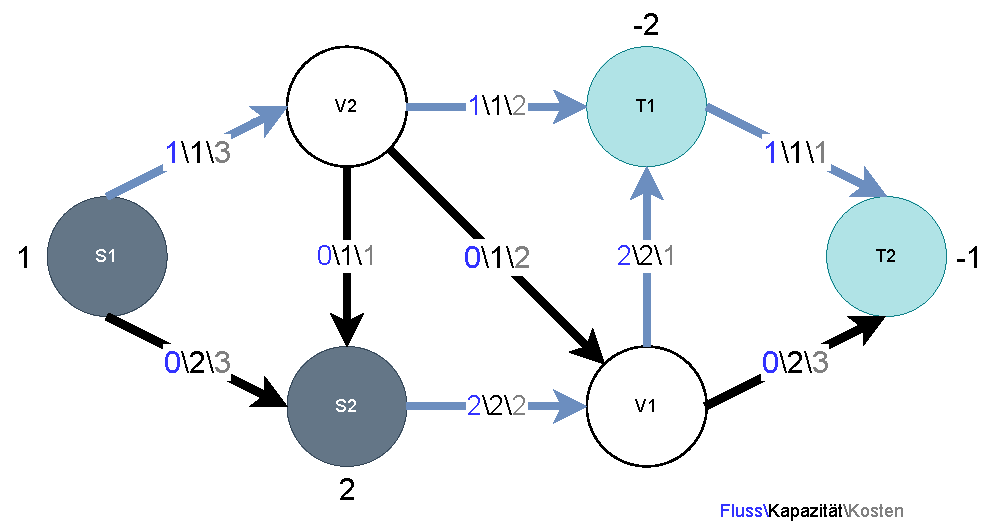
\includegraphics[width=0.7\textwidth]{img/leo/graph1-Page-8.drawio.pdf}
\caption{Cycle-Canceling-Algorithmus Schritt 8}
\label{fig:cc_step8}
\end{figure}

Nun springen wir wieder zu Schritt 2 und erzeugen den Residualgraph mit $u^f$ und $c^f$ zu dem vorigen Graphen (vgl. Abbildung \ref{fig:cc_step9}).
\begin{figure}[htb]
\centering
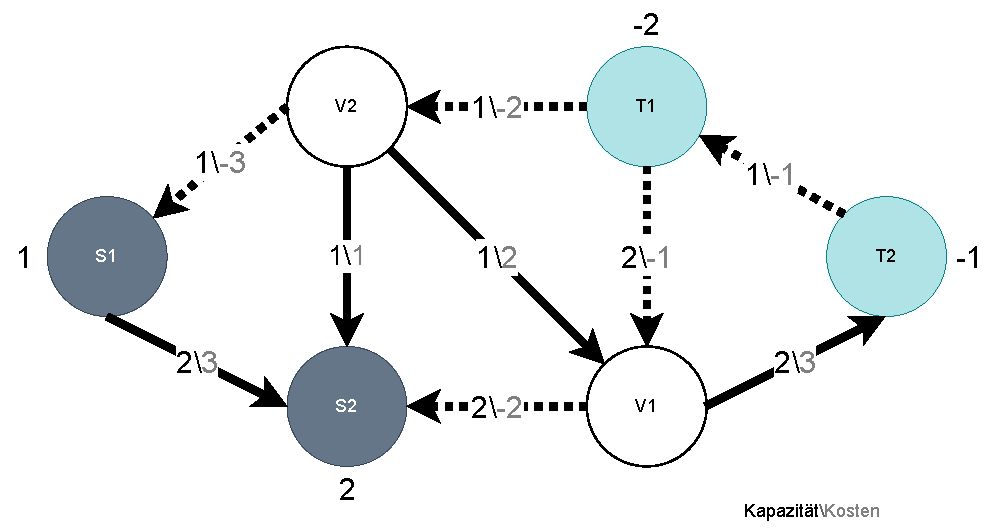
\includegraphics[width=0.7\textwidth]{img/leo/graph1-Page-9.drawio.pdf}
\caption{Cycle-Canceling-Algorithmus Schritt 9}
\label{fig:cc_step9}
\end{figure}

Danach gehen wir wieder zu Schritt 3. über wo wir versuchen, einen $f$-augmentierenden Zykel $Z$ in $G^f$ mit negativen Kosten zu konstruieren. In unserem Beispiel ist kein $f$-augmentierender Zykel $Z$ mit negativen Kosten zu konstruieren. Daraus folgt das wir unseren Algorithmus stoppen, da wir fertig sind. Unser $b$-Fluss ist nun kostenminimal.

\section{Problem des Algorithmus}
Für den Cycle-Canceling-Algorithmus ergibt sich ein ähnliches Problem, welches wir auch schon bei dem Ford-Fulkerson Algorithmus erkannt haben: Die Kosten des kostenminmalen Flusses verbessern sich im schlechtesten Fall immer nur um eine Einheit pro Iteration.

Dieses Problem können wir erneut am Diamantengraphen betrachten. Der Graph hat die Balancen $b(s) = 2N$, $b(t) = -2N$ und $b(v) = 0$. Die oberen Kapazitäten haben alle den Wert $N$ ausgenommen die Kante von $V1$ zu $V2$. Diese Kante hat die obere Kapazität $1$. Die Kosten aller Kanten betragen $0$. Nun erweitern wir den Diamantengraphen noch um eine Kante von $S$ zu $T$. Diese Kante hat die Kosten $1$ und die obere Kapazität $2N$ (vgl. Abbildung \ref{fig:erweiterter_diamantgraph}).

Das Problem wird nun ersichtlich, wenn der Algorithmus im ersten Schritt einen $b$-Fluss erzeugt, für den gilt:
\[ f(e) = \begin{cases}
 2N & $für $ e = (S,T) \\
 0 & $sonst.$
\end{cases} \]

\begin{figure}[htb]
\centering
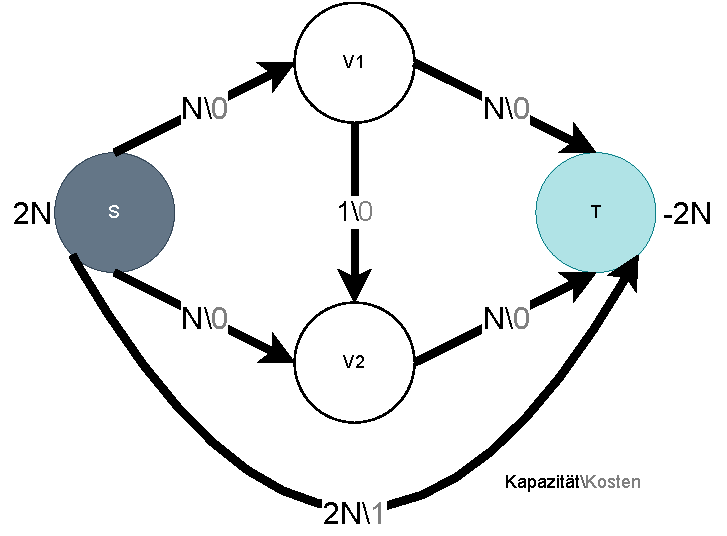
\includegraphics[width=0.7\textwidth]{img/leo/graph1-Page-10.drawio.pdf}
\caption{Erweiterter Diamantgraph}
\label{fig:erweiterter_diamantgraph}
\end{figure}

Anhand des $b$-Fluss (vgl. Abbildung \ref{fig:erweiterter_diamantgraph_mit_fluss}) kann man nun einen Zykel im Residualgraphen erzeugen, sodass mit jeder Iteration sich die Kosten des $b$-Flusses nur um eine Einheit verbessern würden. (vgl. Abbildung \ref{fig:erweiterter_diamantgraph_mit_fluss_res})

\begin{figure}[htb]
\centering
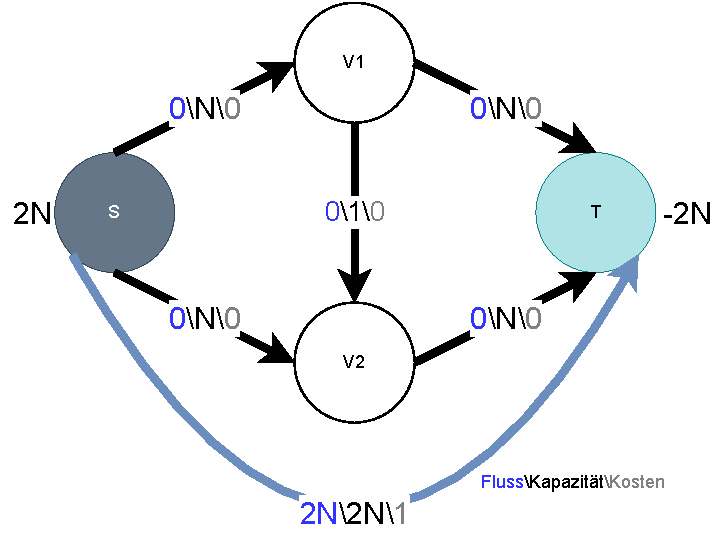
\includegraphics[width=0.7\textwidth]{img/leo/graph1-Page-11.drawio.pdf}
\caption{Erweiterter Diamantgraph mit $b$-Fluss}
\label{fig:erweiterter_diamantgraph_mit_fluss}
\end{figure}

\begin{figure}[htb]
\centering
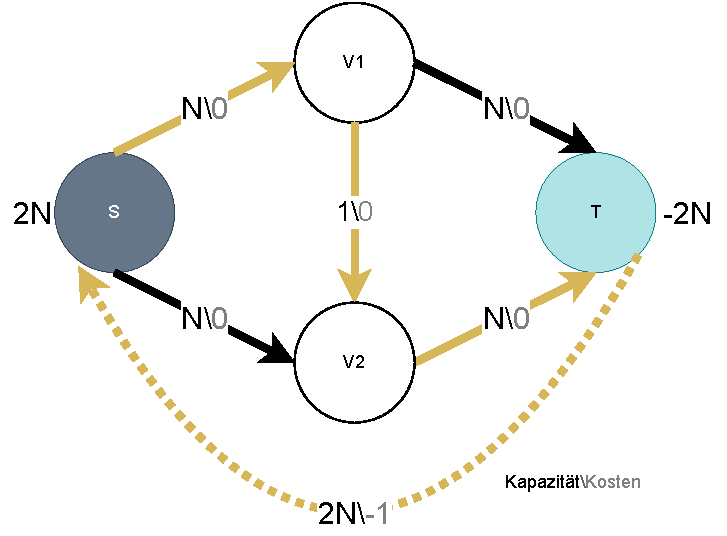
\includegraphics[width=0.7\textwidth]{img/leo/graph1-Page-12.drawio.pdf}
\caption{Residualgraph des erweiterten Diamantgraphen}
\label{fig:erweiterter_diamantgraph_mit_fluss_res}
\end{figure}


\section{Verbesserung des Algorithmus}

Eine Idee, den Algorithmus zu verbessern, wäre bei der Konstruktion des $f$-augmentierten Zykels $Z$ in $G^f$ den Zykel zu konstruieren, der die geringsten Kosten hat. Das Problem, welches sich hierbei jedoch ergibt ist, dass dies dem Problem entspricht einen Hamilton-Kreis zu finden. Eine andere Möglichkeit, die sich deshalb aufgrund der besseren Effizienz anbietet ist, dass man den Zykel mit den geringsten durchschnittlichen Kosten pro Kante wählt. Auch wenn dies schlechter ist als den Zykel mit den geringsten Kosten zu wählen.